\section{问题四:化学成分关联网络与结构差异分析}

古代玻璃的化学成分体系并非各种元素的随机组合,其背后反映了原料选择与烧制工艺的内在规律。为了探寻不同类别玻璃在配方层面的结构性差异,本章将各类玻璃的化学成分体系构建为网络模型。网络中的节点代表化学成分,节点间的连接则代表成分间在配方中存在的直接关联。通过比较高钾玻璃和铅钡玻璃网络的拓扑结构差异,可以探寻其原料与工艺的深层不同。分析过程始于已分类的化学成分数据,首先应用中心化对数比变换处理成分数据固有的统计约束,随后利用图套索算法计算反映成分间直接关联的偏相关系数并构建网络。进一步理解网络的宏观结构,采用社群发现算法对网络节点进行聚类。最终,所有分析结果被整合至可视化网络图中,以呈现两类玻璃在配方结构上的分别特征。

\subsection{成分数据变换与关联构建方法}

玻璃成分数据属于一种特殊的成分数据,其各组分之和恒定。这一特性会在统计上产生闭合效应,引入虚假的负相关关系。例如,当主要成分二氧化硅$SiO_2$的含量增加时,其他所有成分的相对比例必然下降,即使它们在物理化学上并无关联。直接使用传统相关性分析会产生误导性结论。为解决此问题,本研究引入化学计量学领域处理此类数据的核心技术,即中心化对数比变换。该方法通过对数比值变换,将数据投影到一个无约束的几何空间中,从而消除产生虚假负相关的统计基础,保证后续关联性分析的有效性。

对于一个包含$D$种化学成分的样本向量$\boldsymbol{x} = [x_1, x_2, \dots, x_D]$,首先计算其几何平均数$g(\boldsymbol{x})$。
\begin{equation}
g(\boldsymbol{x}) = \left( \prod_{i=1}^{D} x_i \right)^{1/D}
\end{equation}
随后对每个成分$x_i$进行变换,得到新向量$\boldsymbol{y} = \text{clr}(\boldsymbol{x})$的第$i$个元素$y_i$。
\begin{equation}
y_i = \ln\left(\frac{x_i}{g(\boldsymbol{x})}\right)
\end{equation}
在具体计算中,数据中的零值被一个极小的正数替代,以确保对数运算的有效性。

在变换后的数据基础上,需要探寻成分间排除了所有其他成分影响后的直接关联。常规相关系数无法区分直接关系与间接关系,因此需要计算偏相关系数。图套索算法是估计偏相关网络的常用方法,它通过求解一个带$L1$惩罚的优化问题,从数据中估计出一个稀疏的逆协方差矩阵,即精度矩阵,并由此推导出偏相关关系。其目标函数如下。
\begin{equation}
\hat{\Theta} = \arg\max_{\Theta \succ 0} \left( \log(\det\Theta) - \text{tr}(S\Theta) - \lambda \|\Theta\|_1 \right)
\end{equation}
其中,$S$是变换后数据的样本协方差矩阵,$\lambda$是控制稀疏度的正则化参数,$L1$惩罚项会使精度矩阵$\Theta$中许多不重要的元素变为零。得到$\Theta$后,任意两个变量$i$和$j$之间的偏相关系数$\rho_{ij \cdot \text{rest}}$可由以下公式算出。
\begin{equation}
\rho_{ij \cdot \text{rest}} = - \frac{\Theta_{ij}}{\sqrt{\Theta_{ii} \Theta_{jj}}}
\end{equation}
当且仅当$\Theta_{ij}$不等于零时,变量$i$和$j$之间存在直接关联。为避免人工设定正则化参数的主观性,本研究采用交叉验证版本的方法,使其能够自动为不同数据集找到最优的正则化参数。

\subsection{网络社群结构发现}
充满连接的网络图虽然信息量大,但难以直接观察其核心结构。为从更高维度分析网络,本研究引入社群发现算法,其作用是自动识别网络中的模块或社群。一个社群是内部连接远比外部连接紧密的节点集群,在当前背景下可能代表了一组在化学功能或来源上高度相关的成分。本研究选用鲁汶算法,它通过优化模块度指标来迭代地寻找网络的最优社群划分。

\begin{algorithm}[htbp]
	\caption{鲁汶社群发现算法}
	\label{alg:louvain}
	\begin{algorithmic}[1]
		\Require
		\Statex 带权重的图 $G = (V, E, w)$
		\Ensure
		\Statex 节点的社群划分 $P$

		\State 初始化:对于所有节点 $v \in V$,将其分配至独立的社群 $C_v \leftarrow \{v\}$
		\Repeat
			\State 设置标记 $improved \leftarrow \text{false}$
			\State \Comment{第一阶段:节点移动}
			\Repeat
				\State 设置标记 $moved \leftarrow \text{false}$
				\For{每一个节点 $v \in V$}
					\State $C_{current} \leftarrow$ 节点 $v$ 当前所在的社群
					\State $\Delta Q_{max} \leftarrow 0$
					\State $C_{best} \leftarrow C_{current}$
					\For{节点 $v$ 的每一个邻居 $u$}
						\State $C_{neighbor} \leftarrow$ 节点 $u$ 所在的社群
						\If{$C_{neighbor} \neq C_{current}$}
							\State 计算将节点 $v$ 从 $C_{current}$ 移至 $C_{neighbor}$ 的模块度增益 $\Delta Q$
							\If{$\Delta Q > \Delta Q_{max}$}
								\State $\Delta Q_{max} \leftarrow \Delta Q$
								\State $C_{best} \leftarrow C_{neighbor}$
							\EndIf
						\EndIf
					\EndFor
					\If{$C_{best} \neq C_{current}$}
						\State 将节点 $v$ 从 $C_{current}$ 移至 $C_{best}$
						\State $moved \leftarrow \text{true}$
						\State $improved \leftarrow \text{true}$
					\EndIf
				\EndFor
			\Until{$moved = \text{false}$}
			\State \Comment{第二阶段:网络聚合}
			\If{$improved = \text{true}$}
				\State $V' \leftarrow \emptyset$, $E' \leftarrow \emptyset$
				\State 将当前划分中的每个社群 $C$ 视为一个新的超级节点
				\State $V' \leftarrow$ 所有超级节点的集合
				\State 根据原始社群间的连接权重之和,计算超级节点间的边和权重,得到 $E'$
				\State 构建新的聚合图 $G \leftarrow (V', E')$
			\EndIf
		\Until{$improved = \text{false}$}
		\State \Return 当前图 $G$ 中节点的最终社群划分 $P$
	\end{algorithmic}
\end{algorithm}


鲁汶算法是一个多层次的迭代过程。第一阶段为节点移动,初始时每个节点是独立的社群,算法遍历所有节点,尝试将每个节点移动到其邻居所在的社群中,并计算此举带来的模块度增益,节点最终被分配到能使其模块度增益最大的邻居社群中。此过程反复进行,直到没有节点移动能再提升模块度。第二阶段为网络聚合,将第一阶段形成的每个社群压缩成一个超级节点,构建一个新的聚合网络,社群间的连接权重等于原始节点间连接权重的总和。算法重复这两个阶段,直到网络的模块度不再有显著提升,从而得到一个层次化的社群结构。该算法的具体步骤如算法\ref{alg:louvain}所示。


\subsection{两类玻璃化学成分关联网络分析}
最终的关联网络可视化图整合了偏相关强度,社群归属和节点重要性等多个维度的分析结果。图中每个节点代表一种化学成分,节点大小由连接数量与连接强度共同决定,连接广泛且作用强度高的成分由此成为网络的核心枢纽。节点颜色对应其所属的结构社群,颜色相同的节点在配方体系中构成一个功能或来源上相互关联的模块。节点间的连接代表成分间排除了其他变量影响后的直接关联,连接粗细正比于偏相关系数的绝对值,用以表现关联的强度,橙色连接为正相关,青色连接为负相关。

\begin{figure}[htbp]
    \centering
    \begin{minipage}[b]{0.48\textwidth}
        \centering
        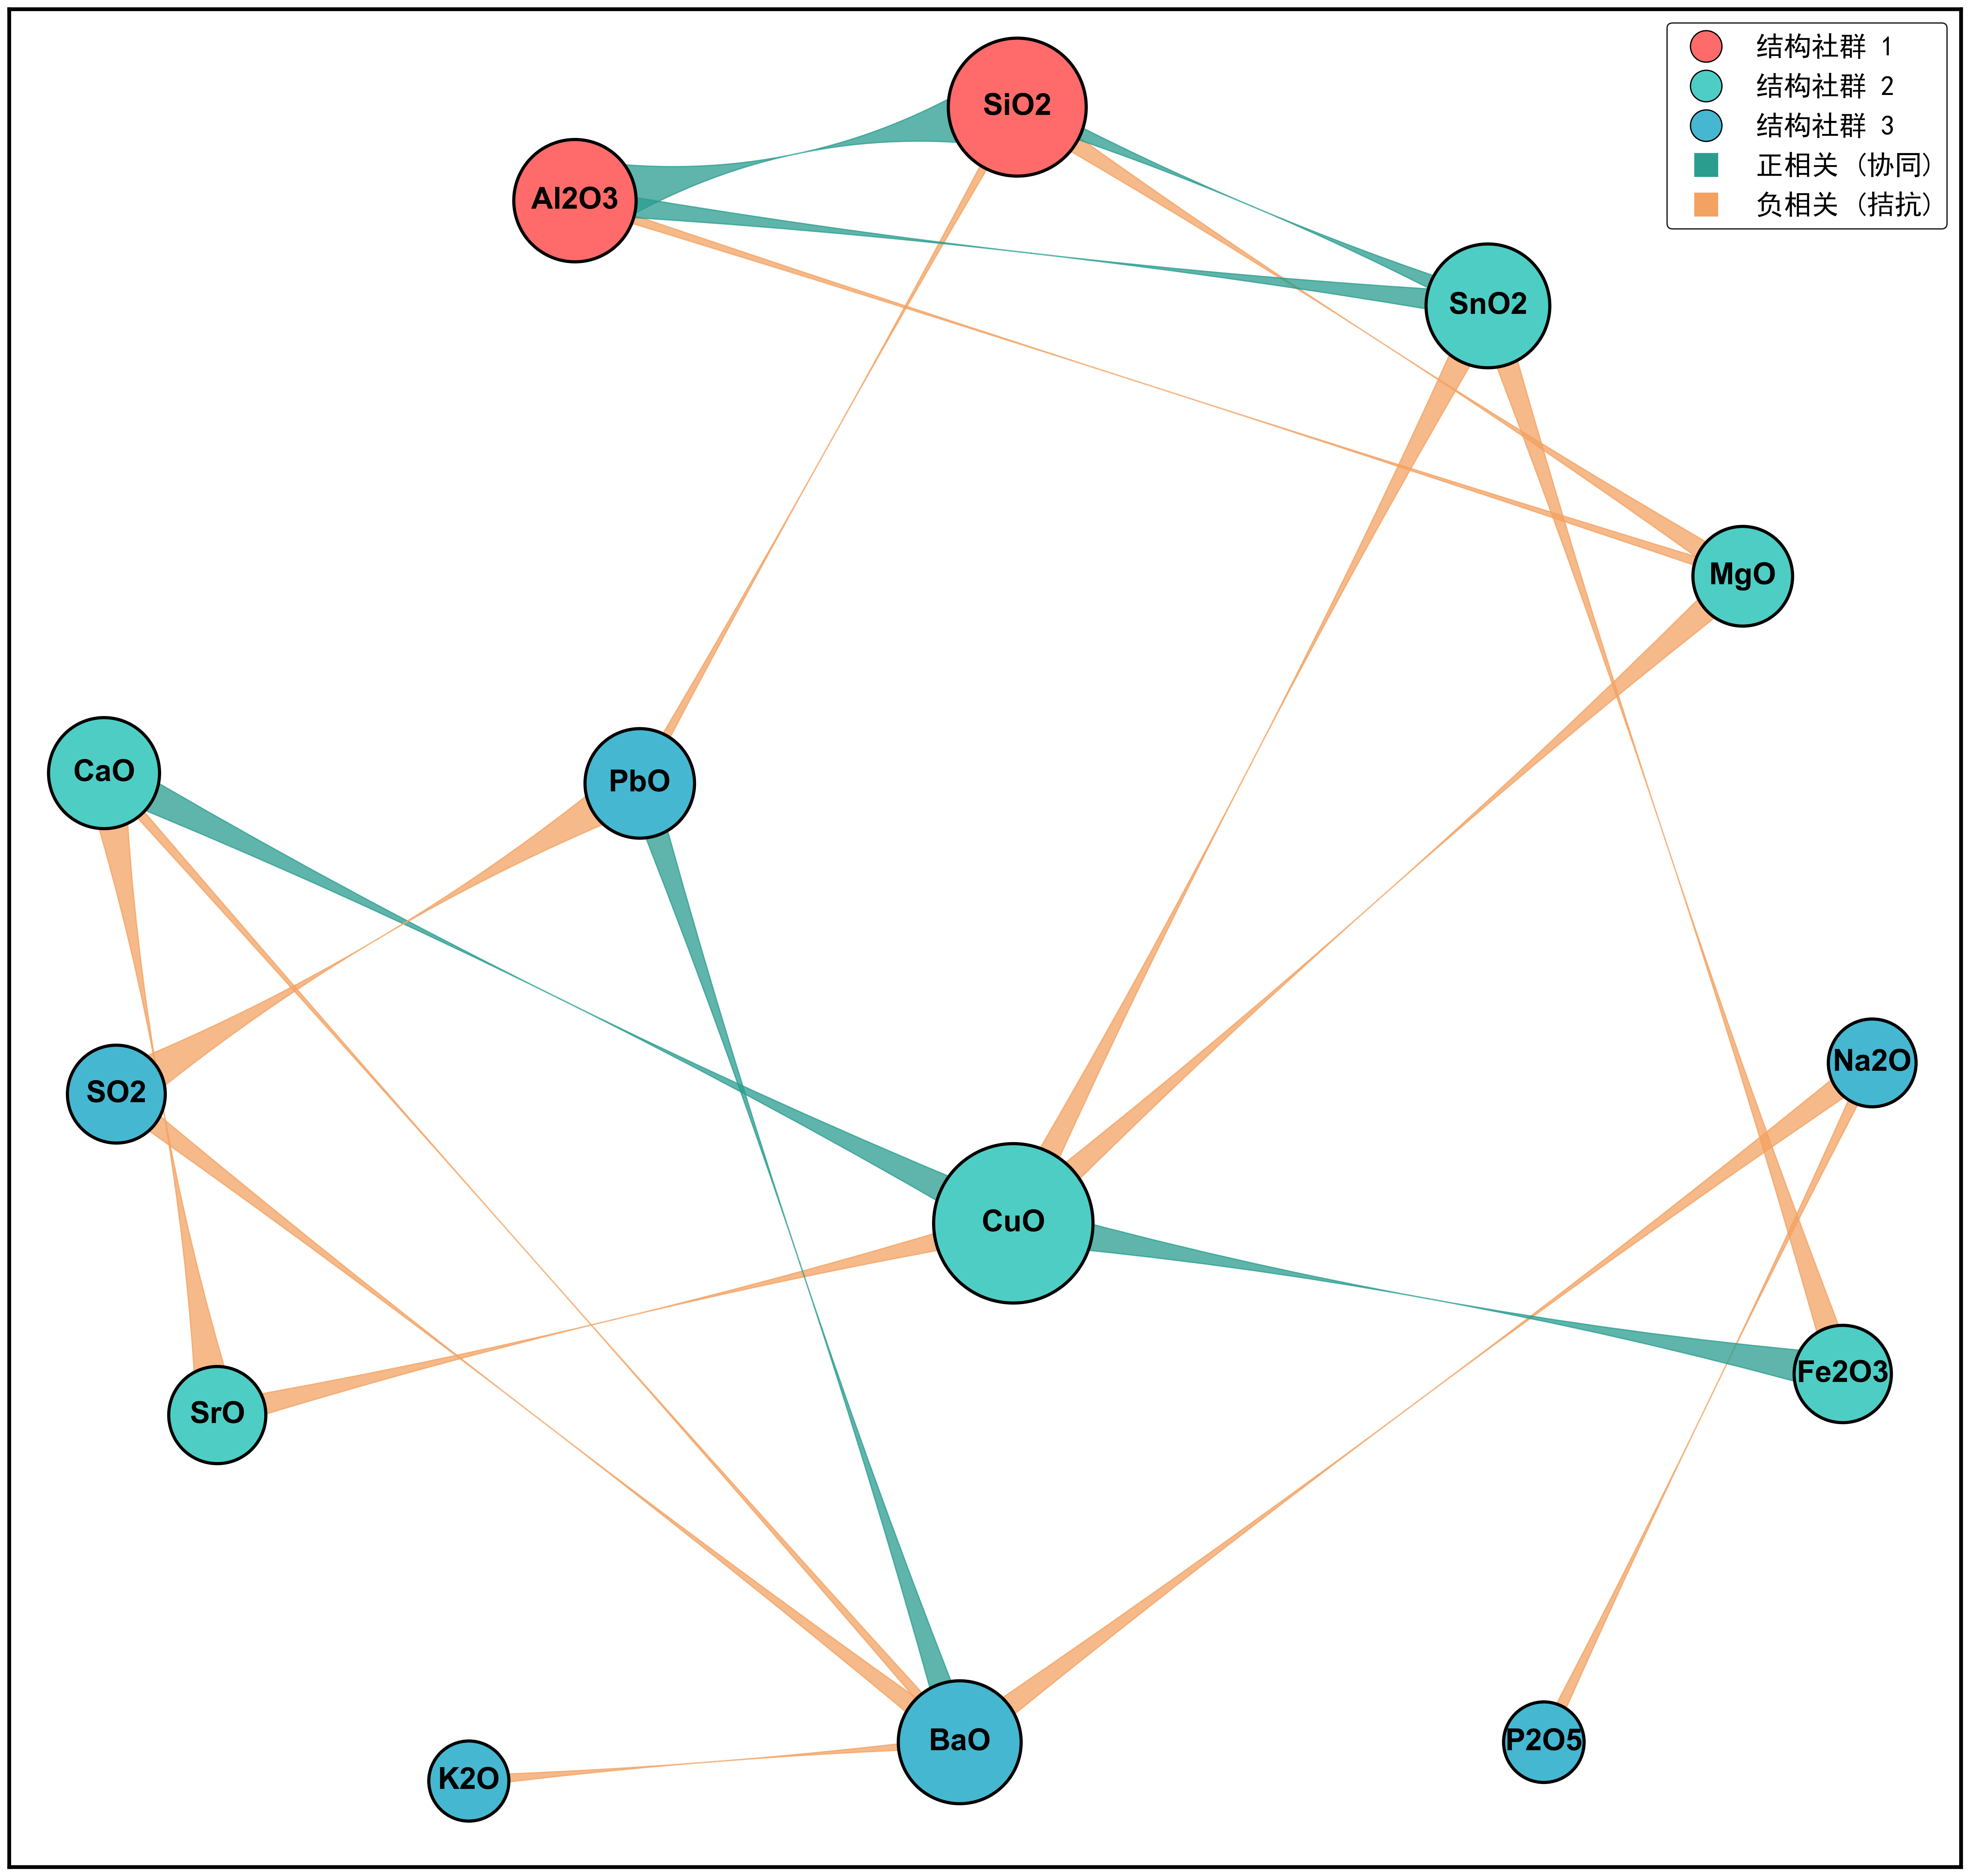
\includegraphics[width=\textwidth]{figs/6问题四/高钾_Network_Final_Soft_Bright.png}
        \caption*{高钾玻璃化学成分关联网络}
    \end{minipage}
    \hfill
    \begin{minipage}[b]{0.48\textwidth}
        \centering
        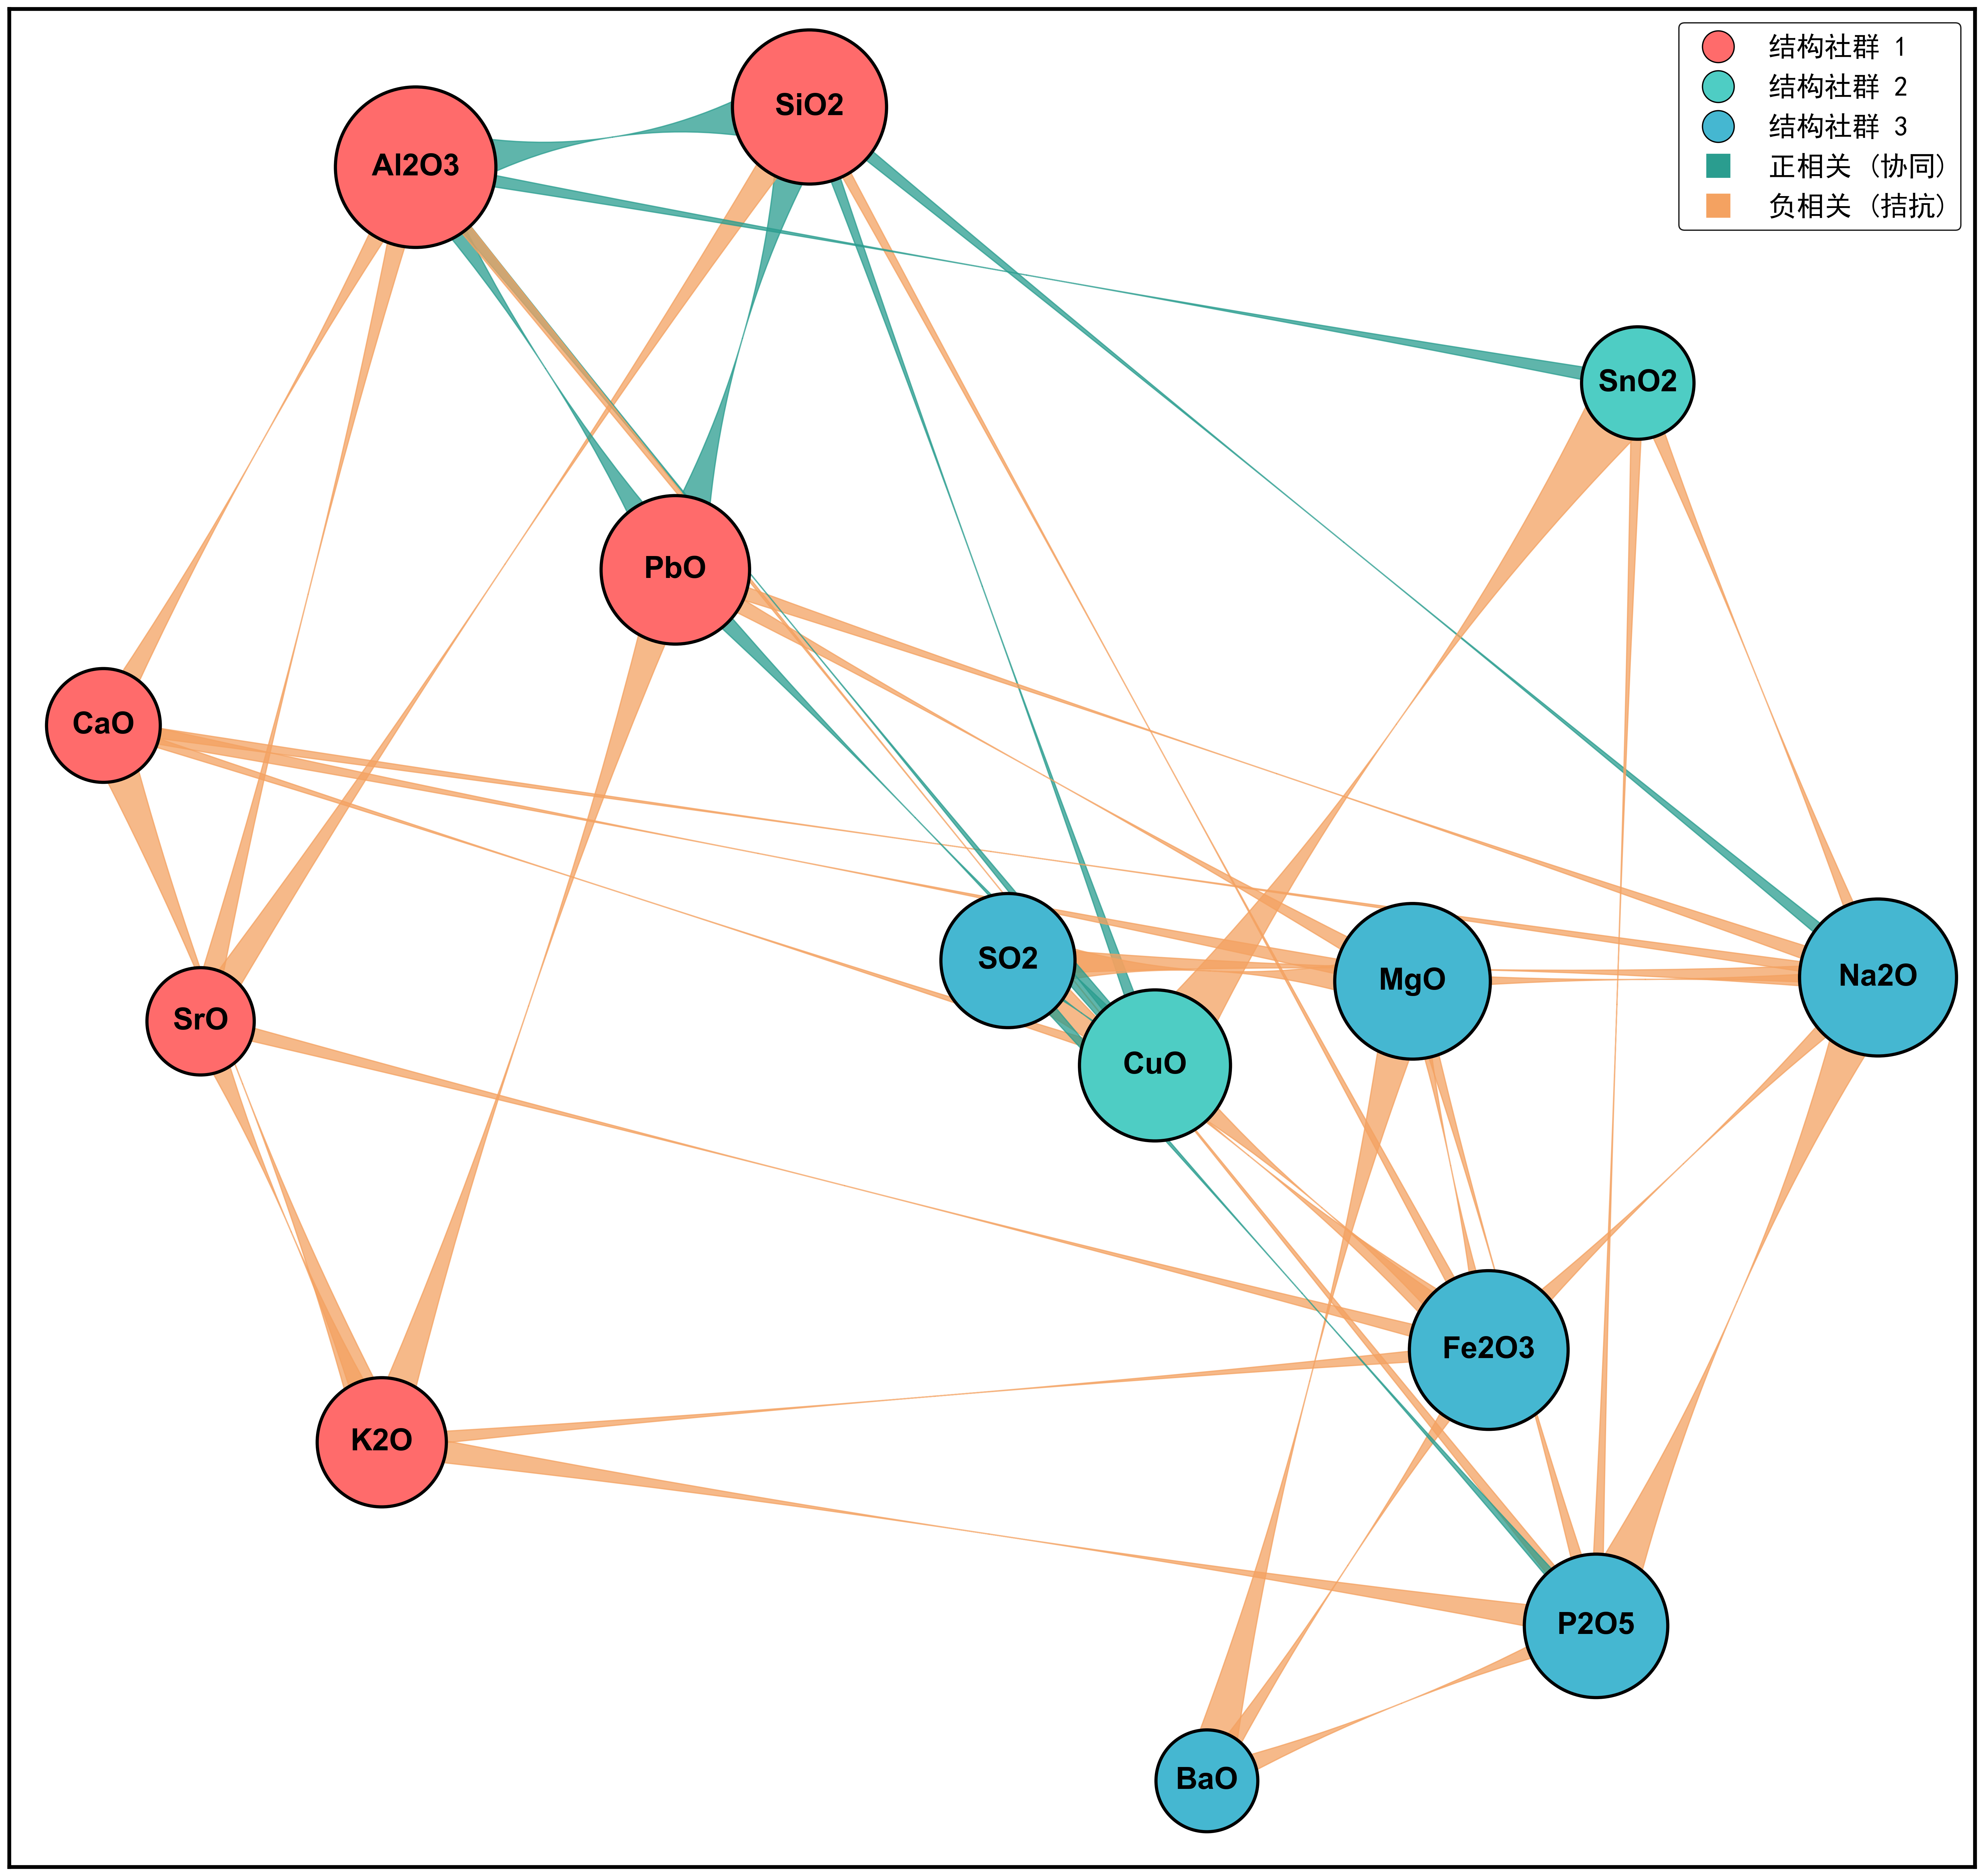
\includegraphics[width=\textwidth]{figs/6问题四/铅钡_Network_Final_Soft_Bright.png}
        \caption*{铅钡玻璃化学成分关联网络}
    \end{minipage}
    \caption{两类玻璃化学成分关联网络对比}
    \label{fig:networks}
\end{figure}

图\ref{fig:networks}A展示了高钾玻璃的化学成分关联网络。其网络结构呈现两个主要社群。社群一为红色,由玻璃主干成分二氧化硅$SiO_2$和氧化铝$Al_2O_3$构成。社群二为青色,包含了氧化铜$CuO$和氧化钡$BaO$在内的多种金属氧化物。一个值得注意的现象是,作为高钾玻璃标志性成分的氧化钾$K_2O$并未归入任何主要社群,这表明在排除了其他成分的普遍影响后,它与其他成分的直接关联不集中。网络中,氧化铜$CuO$,氧化钡$BaO$和二氧化硅$SiO_2$的节点尺寸较大,是网络中的关键节点。从关联上看,二氧化硅$SiO_2$与氧化铅$PbO$之间存在负相关,而氧化铜$CuO$与氧化钡$BaO$之间也表现出负相关关系。

图\ref{fig:networks}B展示了铅钡玻璃的化学成分关联网络。该网络在结构上与高钾玻璃存在显著差异,共形成了三个社群。社群一为红色,是网络的主体,它同时包含了作为玻璃骨架的二氧化硅$SiO_2$和作为助熔剂的氧化铅$PbO$与氧化钾$K_2O$,说明这些成分在配方中协同作用。社群二为青色,主要由氧化钡$BaO$和氧化铁$Fe_2O_3$等成分组成。社群三为蓝色,由氧化锡$SnO_2$和氧化钠$Na_2O$构成。网络的核心节点是氧化铅$PbO$,二氧化硅$SiO_2$和氧化铝$Al_2O_3$。网络中最突出的关联是氧化铅$PbO$与二氧化硅$SiO_2$之间强度很高的正相关,这表明两者在铅钡玻璃的形成过程中有相互促进的作用。与此相对,氧化铝$Al_2O_3$与二氧化硅$SiO_2$之间存在强度较高的负相关。两类玻璃关联网络在社群构成与核心关联上的不同,系统地反映了它们在原料选择与烧制工艺上的区别。

